\documentclass{beamer}

\mode<presentation>
{
  \usetheme{Warsaw}
  \useoutertheme{infolines}
  \usecolortheme{spruce}
  % or ...

  \setbeamercovered{transparent}
  % or whatever (possibly just delete it)
}

\usepackage{hyperref}
\usepackage{multicol}
\usepackage{graphicx}
\usepackage{verbatim}
\usepackage{amsmath}
\usepackage{listings}

\lstloadlanguages{C++}
\lstnewenvironment{code}
	{%\lstset{	numbers=none, frame=lines, basicstyle=\small\ttfamily, }%
	 \csname lst@SetFirstLabel\endcsname}
	{\csname lst@SaveFirstLabel\endcsname}
\lstset{% general command to set parameter(s)
	language=C++, basicstyle=\footnotesize\sffamily, keywordstyle=\slshape,
	emph=[1]{tipo,usa}, emphstyle={[1]\sffamily\bfseries},
	morekeywords={tint,forn,forsn},
	basewidth={0.47em,0.40em},
	columns=fixed, fontadjust, resetmargins, xrightmargin=5pt, xleftmargin=15pt,
	flexiblecolumns=false, tabsize=2, breaklines,	breakatwhitespace=false, extendedchars=true,
	numbers=left, numberstyle=\tiny, stepnumber=1, numbersep=9pt,
	frame=l, framesep=3pt,
}

\usepackage[spanish]{babel}
% or whatever

\usepackage[utf8]{inputenc}
% or whatever

\usepackage{times}
\usepackage[T1]{fontenc}
% Or whatever. Note that the encoding and the font should match. If T1
% does not look nice, try deleting the line with the fontenc.


\title[DP Avanzada] % (optional, use only with long paper titles)
{Temas Avanzados de Programación Dinámica}

\author[Agustín Gutiérrez] % (optional, use only with lots of authors)
{~Agustín Santiago Gutiérrez}
% - Give the names in the same order as the appear in the paper.
% - Use the \inst{?} command only if the authors have different
%   affiliation.
\institute[UBA] % (optional, but mostly needed)
{
  Facultad de Ciencias Exactas y Naturales\\
  Universidad de Buenos Aires
}
\date[TC 2019] % (optional, should be abbreviation of conference name)
{Training Camp Argentina 2020}

% Acá se puede insertar el logo de la UBA
% \pgfdeclareimage[height=0.5cm]{university-logo}{university-logo-filename}
% \logo{\pgfuseimage{university-logo}}



% Delete this, if you do not want the table of contents to pop up at
% the beginning of each subsection:
\AtBeginSubsection[]
{
  \begin{frame}{Contenidos}
  \footnotesize
    \tableofcontents[currentsection, currentsubsection]
  \end{frame}
}

% If you wish to uncover everything in a step-wise fashion, uncomment
% the following command: 

%\beamerdefaultoverlayspecification{<+->}


\begin{document}

\begin{frame}
  \titlepage
\end{frame}

\begin{frame}{Contenidos}
  \tableofcontents
  % You might wish to add the option [pausesections]
\end{frame}

\begin{frame}
  ``Pay heed to the tales of old wives. It may well be that they alone keep in memory what it was once needful for the wise to know.''
  
  \ 
  
  \hfill \textit{J. R. R. Tolkien, The Lord of the Rings}

  \ 
  
  \ 
  
  \ 

``Memory is the thing you forget with.''


  \hfill \textit{Alexander Chase, Perspectives, 1966.}


  \ 
  
  \ 
  
  \ 

``I cannot but remember such things were, \\That were most precious to me.''

  \hfill \textit{William Shakespeare, Macbeth}
  
  \hfill \textit{Act IV, scene 3, line 222}
\end{frame}

\section{Dinámicas con subconjuntos}

\subsection{Idea}

\begin{frame}{Idea}
\begin{itemize}
    \item El estado contiene un \textbf{subconjunto} $S \subseteq T$ de algún conjunto $T$ relevante al problema
    \item Implementación: número de $0$ a $2^n-1$ (máscara de bits: \texttt{0} a \texttt{(1<<n)-1})
       \begin{itemize}
		   \item $\cup$ es el \texttt{|}
		   \item $\cap$ es el \texttt{\&}
		   \item $\{ i \}$ es \texttt{1<<i}
		   \item $T$ es \texttt{(1<<n)-1}
		   \item $\emptyset$ es \texttt{0}
           \item $i \in S$ es \texttt{((1<<i)\&S != 0)} o \texttt{((S>>i)\&1)}
		   \item $S^c$ es \texttt{T\&(\textasciitilde S)} o \texttt{T-S}
		   \item $A - B = A \cap B^c$ es \texttt{A\&(\textasciitilde B)} o \texttt{A\&(T-B)}
       \end{itemize}
    \item Notar que el estado podría tener más cosas, o más de un subconjunto
\end{itemize}
\end{frame}

\subsection{Ejemplos}

\begin{frame}{Ejemplos}
    \begin{itemize}
		\item Matching perfecto de costo mínimo en grafo completo: $O(N2^N)$ [Contest 3: C. Looking for Order]
		\pause
        \invisible<1-1>{
        \item De hecho $O(N\phi^N)$, donde $\phi = \frac{1+\sqrt 5}{2} \approx 1.618$
        }
        \pause
		\invisible<1-2>{
		\item Minimum set cover: $O(M2^N)$, para $M$ conjuntos de $N$ elementos}
        \pause
		\invisible<1-3>{
		\item Bin Packing: $O(N 2^N)$}
		\pause
		\invisible<1-4>{
		\item {\vfill TSP: $O(N^2 2^N)$ \vfill}		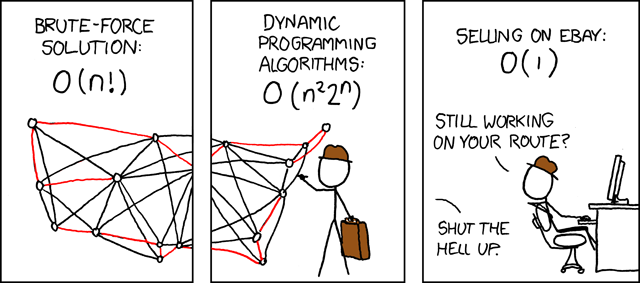
\includegraphics[scale = 0.3]{xkcd.png}
		\item Todas son \textbf{muchísimo} más eficientes que el backtracking directo}
    \end{itemize}
\end{frame}

\section{Tabla aditiva multidimensional}

\subsection{Idea}

\begin{frame}{Sumas parciales (1D)}
    \begin{itemize}
		\item $dp$ se inicializa igual que el vector de entrada 
        \item Se hace \texttt{dp(i) += dp(i-1)} para $i > 0$, en orden
    \end{itemize}
    Con este cómputo $O(N)$ está la suma de todos los \textbf{anteriores}
\end{frame}

\begin{frame}{Sumas parciales (2D)}
    \begin{itemize}
		\item $dp$ se inicializa igual que la matriz de entrada
        \item Se hace \texttt{dp(i,j) += dp(i-1,j)} para $i > 0$, para todos los $j$
        \item \textbf{Luego} se hace \texttt{dp(i,j) += dp(i,j-1)} para $j > 0$, y todo $i$
    \end{itemize}
    Con este cómputo $O(NM)$ está la suma de todos los \textbf{anteriores} en la matriz: $dp(i,j) = \sum_{a=0}^{i} \sum_{b=0}^{j}{v(a,b)}$
    
    \ 
    
    Es exactamente la idea del teorema de Fubini (con sumatorias).
\end{frame}

\begin{frame}{Código multidimensional 5D}
    Ejemplo conceptual para 5 dimensiones. Misma idea, acumular en cada una por separado sucesivamente:
    \begin{itemize}
		\item Poner en $dp$ la entrada
        \item Hacer:\\
        \footnotesize
        \texttt{for dim = 0 to 4}\\
        \texttt{\ for a = 0 to na-1}\\
        \texttt{\ \ for b = 0 to nb-1}\\
        \texttt{\ \ \ for c = 0 to nc-1}\\
        \texttt{\ \ \ \ for d = 0 to nd-1}\\
        \texttt{\ \ \ \ \ for e = 0 to ne-1}\\
        \texttt{\ \ \ \ \ \ pa = a-(dim==0); pb = b-(dim==1); pc = c-(dim==2);}\\
        \texttt{\ \ \ \ \ \ pd = d-(dim==3); pe = e-(dim==4);}\\
        \texttt{\ \ \ \ \ \ if (pa >= 0 \&\& pb >= 0 \&\& pc >= 0 \&\&}\\
        \texttt{\ \ \ \ \ \ \ \ \ \ pd >= 0 \&\& pe >= 0)}\\
        \texttt{\ \ \ \ \ \ \ dp(a,b,c,d,e) += dp(pa,pb,pc,pd,pe)}\\
    \end{itemize}
    Para una matriz de $T$ celdas en total y con $d$ dimensiones, este cómputo $O(T d)$ / $O(T d^2)$ calcula la suma de todos los \textbf{anteriores}
    
    
\end{frame}


\subsection{Ejemplos}

\begin{frame}{Sumas para los subconjuntos}
    \begin{itemize}
		\item Un subconjunto de $T$, que tiene $n$ elementos, es un elemento de una matriz de $2 \times 2 \times \cdots \times 2$ ($n$ veces) [hipercubo]
        \item Esto pues la máscada de bits nos da las $n$ coordenadas, $0$ o $1$
        \item Los subconjuntos de un elemento, son a su vez los anteriores en dicha matriz
        \item Con un for de $1$ a $n$, y luego pasando por los $2^n$ conjuntos haciendo una suma, se computan todas las sumas sobre subconjuntos de
        cada subconjunto: \\
        \texttt{for i = 0 to n-1}\\
        \texttt{\ for mask = 0 to (1<<n) - 1}\\
        \texttt{\ \ if (mask \& (1<<i))}\\
        \texttt{\ \ \ dp(mask) += dp(mask - (1<<i))}\\
        
    \end{itemize}
\end{frame}

\begin{frame}{Sumas para los divisores}
    \begin{itemize}
		\item Sea $S$ es un conjunto cerrado por divisores, y $P$ la lista de primos que aparecen en los números de $S$
        \item Un número tiene $|P|$ coordenadas, los exponentes de los primos.
        \item Los divisores son justamente los ``menores'', vistos con las coordenadas
        \item Se puede sumar los valores sobre los divisores usando la idea de tabla aditiva $|P|$ dimensional:\\
        \texttt{for p $\in$ P}\\
        \texttt{\ for x $\in$ S (DE MENOR A MAYOR)}\\
        \texttt{\ \ if (p divide a x)}\\
        \texttt{\ \ \ dp(x) += dp(x / p)}\\
        
    \end{itemize}
\end{frame}


\section{Dinámicas con frente}

\subsection{Idea}

\begin{frame}{Idea}
    \begin{itemize}
		\item Tenemos que considerar formas de ``llenar'' un tablero.
		\item Como siempre en programación dinámica, queremos ``olvidar lo más posible''
		\item Al ir llenando el tablero, suele alcanzar con saber únicamente la situación en el \textbf{frente} por dónde vamos llenando.
		\item Por ejemplo si queremos llenar un tablero con 0 y 1 pero sin que haya dos 1 pegados:
    \end{itemize}
    $$\begin{array}{cccc}
		? & ? & ? & ? \\
		? & ? & ? & ? \\
		? & ? & ? & ? \\
		? & ? & ? & ? \\
    \end{array}$$
\end{frame}

\begin{frame}{Idea}
    \begin{itemize}
		\item Tenemos que considerar formas de ``llenar'' un tablero.
		\item Como siempre en programación dinámica, queremos ``olvidar lo más posible''
		\item Al ir llenando el tablero, suele alcanzar con saber únicamente la situación en el \textbf{frente} por dónde vamos llenando.
		\item Por ejemplo si queremos llenar un tablero con 0 y 1 pero sin que haya dos 1 pegados:
    \end{itemize}
    $$\begin{array}{cccc}
		\color{red}0 & ? & ? & ? \\
		? & ? & ? & ? \\
		? & ? & ? & ? \\
		? & ? & ? & ? \\
    \end{array}$$
\end{frame}

\begin{frame}{Idea}
    \begin{itemize}
		\item Tenemos que considerar formas de ``llenar'' un tablero.
		\item Como siempre en programación dinámica, queremos ``olvidar lo más posible''
		\item Al ir llenando el tablero, suele alcanzar con saber únicamente la situación en el \textbf{frente} por dónde vamos llenando.
		\item Por ejemplo si queremos llenar un tablero con 0 y 1 pero sin que haya dos 1 pegados:
    \end{itemize}
    $$\begin{array}{cccc}
		\color{red}0 & ? & ? & ? \\
		\color{red}1 & ? & ? & ? \\
		? & ? & ? & ? \\
		? & ? & ? & ? \\
    \end{array}$$
\end{frame}


\begin{frame}{Idea}
    \begin{itemize}
		\item Tenemos que considerar formas de ``llenar'' un tablero.
		\item Como siempre en programación dinámica, queremos ``olvidar lo más posible''
		\item Al ir llenando el tablero, suele alcanzar con saber únicamente la situación en el \textbf{frente} por dónde vamos llenando.
		\item Por ejemplo si queremos llenar un tablero con 0 y 1 pero sin que haya dos 1 pegados:
    \end{itemize}
    $$\begin{array}{cccc}
		\color{red}0 & ? & ? & ? \\
		\color{red}1 & ? & ? & ? \\
		\color{red}0 & ? & ? & ? \\
		? & ? & ? & ? \\
    \end{array}$$
\end{frame}

\begin{frame}{Idea}
    \begin{itemize}
		\item Tenemos que considerar formas de ``llenar'' un tablero.
		\item Como siempre en programación dinámica, queremos ``olvidar lo más posible''
		\item Al ir llenando el tablero, suele alcanzar con saber únicamente la situación en el \textbf{frente} por dónde vamos llenando.
		\item Por ejemplo si queremos llenar un tablero con 0 y 1 pero sin que haya dos 1 pegados:
    \end{itemize}
    $$\begin{array}{cccc}
		\color{red}0 & ? & ? & ? \\
		\color{red}1 & ? & ? & ? \\
		\color{red}0 & ? & ? & ? \\
		\color{red}1 & ? & ? & ? \\
    \end{array}$$
\end{frame}

\begin{frame}{Idea}
    \begin{itemize}
		\item Tenemos que considerar formas de ``llenar'' un tablero.
		\item Como siempre en programación dinámica, queremos ``olvidar lo más posible''
		\item Al ir llenando el tablero, suele alcanzar con saber únicamente la situación en el \textbf{frente} por dónde vamos llenando.
		\item Por ejemplo si queremos llenar un tablero con 0 y 1 pero sin que haya dos 1 pegados:
    \end{itemize}
    $$\begin{array}{cccc}
		0 & \color{red}1 & ? & ? \\
		\color{red}1 & ? & ? & ? \\
		\color{red}0 & ? & ? & ? \\
		\color{red}1 & ? & ? & ? \\
    \end{array}$$
\end{frame}

\begin{frame}{Idea}
    \begin{itemize}
		\item Tenemos que considerar formas de ``llenar'' un tablero.
		\item Como siempre en programación dinámica, queremos ``olvidar lo más posible''
		\item Al ir llenando el tablero, suele alcanzar con saber únicamente la situación en el \textbf{frente} por dónde vamos llenando.
		\item Por ejemplo si queremos llenar un tablero con 0 y 1 pero sin que haya dos 1 pegados:
    \end{itemize}
    $$\begin{array}{cccc}
		0 & \color{red}1 & ? & ? \\
		1 & \color{red}0 & ? & ? \\
		\color{red}0 & ? & ? & ? \\
		\color{red}1 & ? & ? & ? \\
    \end{array}$$
\end{frame}

\begin{frame}{Idea}
    \begin{itemize}
		\item Tenemos que considerar formas de ``llenar'' un tablero.
		\item Como siempre en programación dinámica, queremos ``olvidar lo más posible''
		\item Al ir llenando el tablero, suele alcanzar con saber únicamente la situación en el \textbf{frente} por dónde vamos llenando.
		\item Por ejemplo si queremos llenar un tablero con 0 y 1 pero sin que haya dos 1 pegados:
    \end{itemize}
    $$\begin{array}{cccc}
		0 & \color{red}1 & ? & ? \\
		1 & \color{red}0 & ? & ? \\
		0 & \color{red}0 & ? & ? \\
		\color{red}1 & ? & ? & ? \\
    \end{array}$$
\end{frame}

\begin{frame}{Idea}
    \begin{itemize}
		\item Tenemos que considerar formas de ``llenar'' un tablero.
		\item Como siempre en programación dinámica, queremos ``olvidar lo más posible''
		\item Al ir llenando el tablero, suele alcanzar con saber únicamente la situación en el \textbf{frente} por dónde vamos llenando.
		\item Por ejemplo si queremos llenar un tablero con 0 y 1 pero sin que haya dos 1 pegados:
    \end{itemize}
    $$\begin{array}{cccc}
		0 & \color{red}1 & ? & ? \\
		1 & \color{red}0 & ? & ? \\
		0 & \color{red}0 & ? & ? \\
		1 & \color{red}0 & ? & ? \\
    \end{array}$$
\end{frame}

\begin{frame}{Idea}
    \begin{itemize}
		\item Tenemos que considerar formas de ``llenar'' un tablero.
		\item Como siempre en programación dinámica, queremos ``olvidar lo más posible''
		\item Al ir llenando el tablero, suele alcanzar con saber únicamente la situación en el \textbf{frente} por dónde vamos llenando.
		\item Por ejemplo si queremos llenar un tablero con 0 y 1 pero sin que haya dos 1 pegados:
    \end{itemize}
    $$\begin{array}{cccc}
		0 & 1 & \color{red}0 & ? \\
		1 & \color{red}0 & ? & ? \\
		0 & \color{red}0 & ? & ? \\
		1 & \color{red}0 & ? & ? \\
    \end{array}$$
\end{frame}

\begin{frame}{Idea}
    \begin{itemize}
		\item Tenemos que considerar formas de ``llenar'' un tablero.
		\item Como siempre en programación dinámica, queremos ``olvidar lo más posible''
		\item Al ir llenando el tablero, suele alcanzar con saber únicamente la situación en el \textbf{frente} por dónde vamos llenando.
		\item Por ejemplo si queremos llenar un tablero con 0 y 1 pero sin que haya dos 1 pegados:
    \end{itemize}
    $$\begin{array}{cccc}
		0 & 1 & \color{red}0 & ? \\
		1 & 0 & \color{red}0 & ? \\
		0 & \color{red}0 & ? & ? \\
		1 & \color{red}0 & ? & ? \\
    \end{array}$$
\end{frame}

\begin{frame}{Estado}
    \begin{itemize}
		\item El estado tendrá la posición $(x,y)$ actual en el tablero.
		\item Además, para un tablero de $N \times M$, guardará $N$ valores (o a veces $N+1$) con el frente.
		\item Si los valores son binarios como en el ejemplo hay $O(NM2^N)$ estados, pero en cambio hay $2^{NM}$ tableros.
	\end{itemize}
\end{frame}


\subsection{Ejemplos}

\begin{frame}{Ejemplos}
    \begin{itemize}
		\item Cantidad de maneras de cubrir con dominós, un tablero con agujeros en posiciones dadas
		\pause
		\invisible<1>{
		\item Cantidad de maneras de cubrir con ``tuberías'' cerradas (ciclos), un tablero con agujeros en posiciones dadas \\
		{\hfill 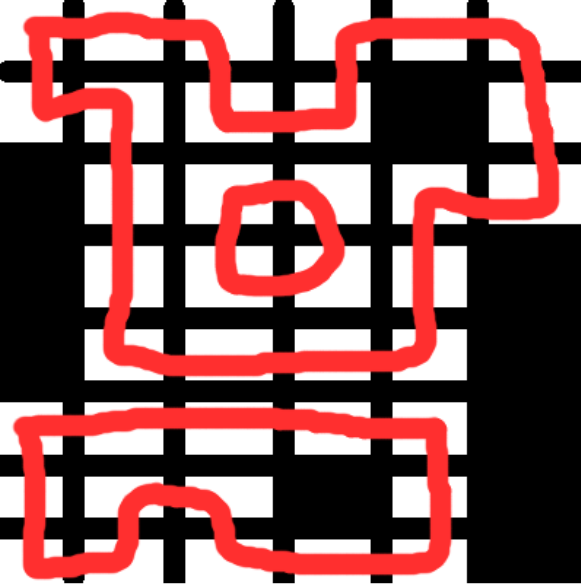
\includegraphics[scale = 0.2]{tuberias.png} \hfill}
		}
		\pause
		\invisible<1-2>{
		\item El frente anterior tiene $O(2^N)$ valores posibles. ¿Y si quisiéramos saber la mínima cantidad de ciclos necesarios?
		}
		\pause
		\invisible<1-3>{
		\item Se puede con un frente con $O(3^N)$ valores posibles (desafío)
		}
    \end{itemize}
\end{frame}

\begin{frame}{Ejemplo final: pintar mural}
    \begin{itemize}
		\item Hay un mural (grilla con obstáculos). Podemos hacer pintadas verticales u horizontales. Podemos pasar varias veces por la misma casilla, pero nunca por un obstáculo. Calcular mínima cantidad de pinceladas para pintar todas las casillas sin obstáculo.
        
        {\hfill 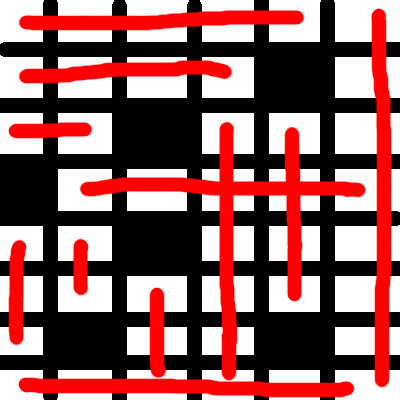
\includegraphics[scale=0.25]{pintapatio.png} \hfill}
        
        \ 
    \end{itemize}
\end{frame}

\begin{frame}{Ejemplo final: pintar mural}
    \begin{itemize}
		\item También se puede resolver con una DP con frente: $O(NM2^N)$
		\pause
		\invisible<1-1>{
		\item Existe en este caso una solución polinomial con matching máximo bipartito:
        
        {\hfill 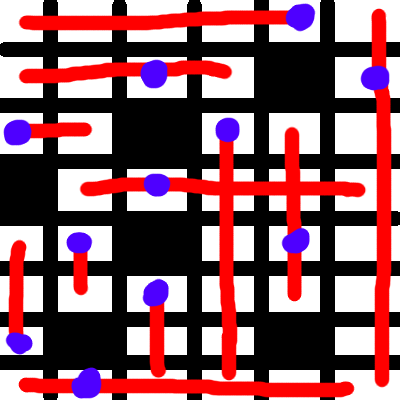
\includegraphics[scale=0.25]{pintapatio2.png} \hfill}
        
		}
    \end{itemize}
\end{frame}

\section{Algunas optimizaciones de DP}

\subsection{Convex Hull Trick}

\begin{frame}{CHT aplicado a DP}
    \begin{itemize}
		\item Ya vimos en otra charla que CHT es una técnica e idea geométrica independiente de DP, que responde queries.
        \item Es muy común sin embargo usar esta estructura para optimizar algoritmos de DP.
    \end{itemize}
\end{frame}

\begin{frame}{CHT aplicado a DP: Ejemplos}
    \begin{itemize}
            \item Tengo $N$ vendedores ordenados en fila. Cada vendedor tiene un entero $a_i$ (posiblemente negativo). Yo voy pasando y a algunos les compro. Si le compro al $i$, obtengo un beneficio $i^2 a_j$, donde $j$ es el comerciante anterior al cual le compré (o bien $a_j=0$ si es a $i$ al primero que compro). ¿Cuál es el máximo beneficio posible?
            \pause
            \invisible<1-1>{
                \item Propuesta: \texttt{dp[j] = } ``Beneficio óptimo de los siguientes comerciantes, si empiezo comprando en el $j$''
                \item Propuesta: $dp(j) = max_{i=j+1}^{n}{\ i^2 a_j + dp(i)}$
                \pause
                \invisible<1-2>{
                \item Si a medida que calculo voy insertando las rectas $y = i^2 x + dp(i)$ (que están ordenadas por pendiente) queda $O(N \lg N)$ con CHT
                }
            }
            \pause
            \invisible<1-3>{
                \item Otro ejemplo: Problema K. The Fair Nut and Rectangles del contest 3.
            }
    \end{itemize}
\end{frame}


\subsection{``Alien Trick'' (AKA multiplicador de Lagrange)}

\begin{frame}{¿Qué es Alien Trick? Un poco de historia}
    \begin{itemize}
		\item Es una idea muy ingeniosa para reemplazar un parámetro de DP, por una búsqueda binaria.
        \item Se la conoce así porque ``se volvió viral'' con el problema Aliens de la IOI Rusia 2016.
        \item La técnica ya era conocida desde antes, aunque casi no se usaba en programación competitiva:
        \pause
        \invisible<1-1>{
            \begin{itemize}
                \item Se menciona en ``Apuntes de Programación Dinámica 1995'' de Fabio Vicentini, FCEN-UBA
                \pause
        \invisible<1-2>{
                \item Tiene una estrecha relación con los archi-conocidos multiplicadores de Lagrange, por lo que en algunos textos matemáticos se encuentra con ese nombre.
                }
                \pause
        \invisible<1-3>{
                \item En otros textos en cambio, se le llamaría Parameter Search.
                }
                \pause
        \invisible<1-4>{
                \item Los competidores de olimpíadas chinos ya conocían y usaban este truquito desde antes y lo llamaban ``wqs binary search'', pues el competidor wqs lo contó en un training camp chino y se volvió popular allí.
                }
            \end{itemize}
            }
    \end{itemize}
\end{frame}

\begin{frame}{Problema de ejemplo para fijar ideas}
    \begin{itemize}
		\item Supongamos el siguiente problema: dado un arreglo de $n$ números distintos, separarlo en \textbf{a lo sumo} $k$ subarreglos minimizando la suma de las diferencias (absolutas) \textbf{entre elementos consecutivos en un mismo subarreglo}.
        \item Este problema es fácil de resolver golosamente en $O(n \lg n)$, pero lo ignoraremos para tener un ejemplo fácil de entender.
        \item Podemos plantear $dp(n,k)$ como antes y queda $dp(n,k) = min(dp(n-1,k-1), dp(n-1,k) + |a_n - a_{n-1}|)$, de complejidad $O(nk)$.
        \item Utilizaremos la técnica de multiplicador de Lagrange para acelerar esta $dp$.
    \end{itemize}
\end{frame}

\begin{frame}{Idea central}
    \begin{itemize}
		\item La idea central es eliminar por completo el parámetro $k$, pero \textbf{introducir un costo $\lambda \geq 0$ por cada subarreglo} que se usa.
        \item Así, el nuevo problema $f_\lambda(n)$ es la forma óptima de partir los primeros $n$ en subarreglos:
            \begin{itemize}
                \item La cantidad ya no está restringida, es libre.
                \item Pero cada subarreglo distinto implica un costo $\lambda$
                \item DP lineal: $f_{\lambda}(n) = min(f_{\lambda}(n-1) + \lambda, f_{\lambda}(n-1) + |a_n - a_{n-1}|)$
            \end{itemize}
        %\item En general con cualquier dp similar: $f_\lambda(n) = min_{k=1}^{n}{f(n,k) - \lambda k}$
        \item Intuitivamente, transformamos una \textbf{restricción} estricta, en un simple \textbf{costo} ajustable $\lambda$.
        \item ¿Para qué sirve este nuevo problema?
    \end{itemize}
\end{frame}

\begin{frame}{Lemas fundamentales}
    \begin{itemize}
		\item Notamos $k_\lambda(n)$ a la cantidad de subarreglos que utiliza una solución óptima para el problema $f_\lambda(n)$ (argmin en diapo previa).
        \item $k_\lambda$ se puede calcular en la misma dp lineal de $f_\lambda$
        \item Las funciones $f_\lambda$ y $k_\lambda$ tienen propiedades clave:
         \pause
          \invisible<1-1>{
            \begin{itemize}
                \item Si $0 \leq \lambda < \mu$ entonces $k_\lambda \geq k_\mu$ (``más caros, menos uso'')
                \pause
                \invisible<1-2>{
                    \item Si $x$ es una solución óptima de $f_\lambda(n)$, entonces $x$ es una solución óptima de $f(n, k_\lambda(n))$
                }
            \end{itemize}
        }
    \end{itemize}
\end{frame}

\begin{frame}{Utilidad de los lemas fundamentales}
    \begin{itemize}
		\item Por el segundo lema, si encontramos algún $\lambda$ tal que $k_\lambda(n)$ tome el valor $k$ de nuestro problema original, la solución que encontramos al calcular $f_\lambda$ es óptima para el problema original.
        \pause
        \invisible<1-1>{f
            \item ¡Pero por el primer lema, se puede buscar tal $\lambda$ con búsqueda binaria!
            \item La complejidad final resulta entonces $N \lg MAX$
        }
    \end{itemize}
\end{frame}

\begin{frame}{Pero hay un problema...}
    \begin{itemize}
		\item En la explicación anterior se asume que va a existir un $\lambda$ tal que $k_\lambda$ tenga el valor que deseamos.
        \item Si existe, lo vamos a encontrar y ya sabemos que la respuesta va a ser óptima. Pero en general, podría no existir...
        \pause
        \invisible<1-1>{f
            \item Teorema: Si $a(k) = $ ``Solución al problema usando \textbf{exactamente} $k$ subarreglos'' es estrictamente convexa como función de $k$, entonces existe el $\lambda$ deseado.
            \item Estrictamente convexa significa $a(k+1) - a(k) < a(k+2) - a(k+1)$ (``derivada creciente'')
            \item Intuitivamente: Cada subarreglo adicional que nos dan tiene que ser ``menos útil'' que el anterior.
            \item Si la función es convexa aunque no estrictamente, hay que tener cierto cuidado pero aún puede utilizarse la misma técnica.
        }
    \end{itemize}
\end{frame}


\begin{frame}{Sobre convexidad}
    \begin{itemize}
		\item Como casi siempre en optimización de DP, demostrar la convexidad no siempre es fácil.
        \item Pero casi siempre es posible convencerse bastante intuitivamente. 
    \end{itemize}
\end{frame}

\begin{frame}{Multiplicador de Lagrange (en general)}
    \begin{itemize}
		\item Ahora que vimos el ejemplo y la idea general, plantiemos lo mismo un poco más en general.
        \item Buscamos una solución $x$ en un espacio de posibles soluciones $X$
        \item Llamamos $f(x)$ al costo que buscamos minimizar
        \item Hay una función $h(x) > 0$ de \textbf{restricción}, que generalmente mide ``cuánto recurso usamos''
        \item Llamamos $a(k) = min_{h(x)=k}{f(x)}$ (valor de la mejor solución que ``usa una cantidad $k$ de recurso'')
        \item En general lo que buscamos calcular es $a(k)$, o a veces el análogo con $h(x) \leq k$
    \end{itemize}
\end{frame}

\begin{frame}{Multiplicador de Lagrange (cont.)}
    \begin{itemize}
		\item Definimos $f_\lambda(x) = f(x) + \lambda h(x)$, para $\lambda \geq 0$
        \item De las definiciones anteriores, una expresión para el valor óptimo es $f_\lambda$ es:
                $opt(\lambda) = f_\lambda(x_{optimo}) = min_{k=1}^{n}{a(k) + \lambda k}$
        \item Llamamos $k_\lambda$ al menor valor posible de $k$ en el que se alcanza el mínimo de la fórmula anterior
        \item Los lemas fundamentales son:
            \begin{itemize}
                \item $opt(\lambda)$ es estrictamente creciente
                \item Si $0 \leq \lambda < \mu$ entonces $k_\lambda \geq k_\mu$
                \item Si $opt(\lambda) = f_\lambda(x_{optimo})$, entonces $x_{optimo}$ es una solución óptima para el problema $min_{h(x) \leq h({x_{optimo}})} f(x)$
            \end{itemize}
    \end{itemize}
\end{frame}

\begin{frame}{Existencia de $\lambda$}
    \begin{itemize}
		\item ¿Cuándo podemos garantizar que habrá un $\lambda$ adecuado?
        \item La clave está en analizar cuándo se reduce $k_\lambda$
        \item Si $k_\lambda = t$, de $opt(\lambda) = min_{k=1}^{n}{a(k) + \lambda k}$  se deduce que $k_\lambda$ cambiará cuando sea $a(t-1) - a(t) \leq \lambda$
        \item Si $a$ es estrictamente convexa, estas condiciones se cumplen todas en distintos valores de $\lambda$, así que $k_\lambda$ pasa por todos los valores.
        \item También se observa que si $a$ toma valores enteros, entonces basta con probar valores enteros de $\lambda$.
        
    \end{itemize}
\end{frame}

\begin{frame}{Caso $a$ convexa no estricta}
    \begin{itemize}
        \item Si la función $a$ es convexa no estrictamente, puede pasar $k_\lambda - k_{\lambda+1} > 1$.
        \item En ese caso, todos los $k$ que cumplen $k_{\lambda+1} \leq k \leq k_\lambda$
            optimizan $f_\lambda$, así que sus valores coinciden con el calculado la obtener $k_{\lambda+1}$
        \item Esto permite calcular los distintos $a(k)$ en este rango, pues forman una progresión aritmética con diferencia $\lambda$.
        \item Reconstruir la solución y no solo el valor en este caso puede ser un problema más complicado, ya que tenemos la dp ejecutada que obtuvo un cierto $k$, pero queremos otro.
    \end{itemize}
\end{frame}

\begin{frame}{Patrón general (resumen)}
    \begin{itemize}
		\item Tenemos una clásica dp del estilo $dp(n,k) = $ ``Forma óptima de resolver para los $n$ primeros elementos, usando \textbf{a lo sumo} $k$''
        \item Nos queda una DP $O(nk^2)$, con suerte $O(nk)$, pero ya no podemos bajar más a menos que cambiemos el estado.
        \item Solución: Introduciendo un multiplicador de Lagrange $\lambda$, reducimos el estado a solamente $dp(n)$, pero pudiendo controlar el $k$ mediante búsqueda binaria variando $\lambda$.
    \end{itemize}
\end{frame}

\begin{frame}{Lectura adicional}
    \begin{itemize}
        \item \url{http://serbanology.com/show_article.php?art=The\%20Trick\%20From\%20Aliens}
        \item \url{https://codeforces.com/blog/entry/68778}
        \item \url{https://ioinformatics.org/files/ioi2016solutions.pdf}
		\item \url{https://codeforces.com/blog/entry/49691}
        \item Problema Aliens para intentar: \url{https://wcipeg.com/problem/ioi1623}
    \end{itemize}
\end{frame}


\section{Optimizaciones de DP basadas en argmin monótono (Bonus, solo si sobra tiempo)}

\subsection{Optimización de Knuth}

\begin{frame}{Ejemplo motivador}
    \begin{itemize}
		\item Dados $n$ valores enteros distintos $v_i$, junto a sus frecuencias $f_i$, dar un árbol binario de búsqueda óptimo para los valores.
		\pause
		\invisible<1>{
			\item $dp(i,j) = \mbox{min}_{k=i}^{j-1}{\ dp(i,k) + dp(k+1,j) + sum_f(i,j)}$
			\item Complejidad: $O(n^3)$
			\item ¿Se podrá mejorar?
		}
    \end{itemize}
\end{frame}

\begin{frame}{Contexto}
    \begin{itemize}
		\item ¡Sí! Con la optimización de Knuth
		\item Dado un algoritmo de dp de dos parámetros cualquiera, es decir \\ $dp(i,j)$ con $0 \leq i, j \leq N$ (ejemplo $i \leq j$ si es \textbf{DP en rangos})
		\item Si su recursión tiene la forma $dp(i,j) = \underset{k}{\mbox{min}}{\ g(i,j, k)}$ para cierta $g$ que solo usa valores $dp(a,b)$ con $a \geq i$ y con $b \leq j$
		\item Podemos definir $K(i,j)$ como el menor $k$ en donde se alcanza el mínimo de la expresión para $dp(i,j)$
        \item Para escribir las complejidades, notaremos $|K|$ a la cantidad de valores posibles para $k$ en la expresión. Típicamente $|K|$ es aproximadamente $N$
        \item En las típicas dp en rango, $k$ se mueve entre $i$ y $j$.
    \end{itemize}
\end{frame}

\begin{frame}{Condición de Knuth}
    \begin{itemize}
		\item $K(i,j-1) \leq K(i,j) \leq K(i+1, j)$
		\item Equivalentemente: $K$ es \textbf{monótona en ambos parámetros}.  
        \item En criollo para DPs en rangos:
		  \begin{itemize}
			\item Si agregamos un elemento por \textbf{izquierda}, \\ el $K$ se mueve \textbf{a la izquierda}
			\item Si agregamos un elemento por \textbf{derecha}, \\ el $K$ se mueve \textbf{a la derecha}
		  \end{itemize}
        \item Llamamos a la anterior la \textit{Condición de Knuth}
		\item Suele ser mucho más difícil demostrar que se cumple, que convencerse o intuir que así será
    \end{itemize}
\end{frame}

\begin{frame}{Optimización de Knuth}
    \begin{itemize}
		\item Como vale la condición de Knuth, es muy simple cambiar en el código la recursión usando las cotas para iterar menos:
		\item $dp(i,j) = \mbox{min}_{k=K(i,j-1)}^{K(i+1,j)}{\ g(i,j,k)}$
		\item Los $K$ los podemos ir calculando en el mismo algoritmo junto a los valores $dp$.
		\item Las cotas sirven para iterar menos... ¿Pero estamos mejorando la complejidad asintótica?
		\pause
		\invisible<1>{
			\item Teorema: Con este sencillísimo cambio al código básico, el algoritmo es $O(N (N+|K|))$ (la cota anterior era $O(N^2 |K|$)
			\item Demostración: La sumatoria de los costos es telescópica en 2D (dibujos)
			\item Si evaluar $g$ no es $O(1)$, el costo son $O(N(N+|K|))$ llamadas a $g$
		}
    \end{itemize}
\end{frame}

\begin{frame}{Optimización de Knuth (dibujos)}
    \begin{itemize}
		\item Costo para calcular $dp(i,j)$: \color{red}$K(i+1,j)\color{black} - \color{green}K(i,j-1)\color{black} + 1$
    \end{itemize}
    {\hfill 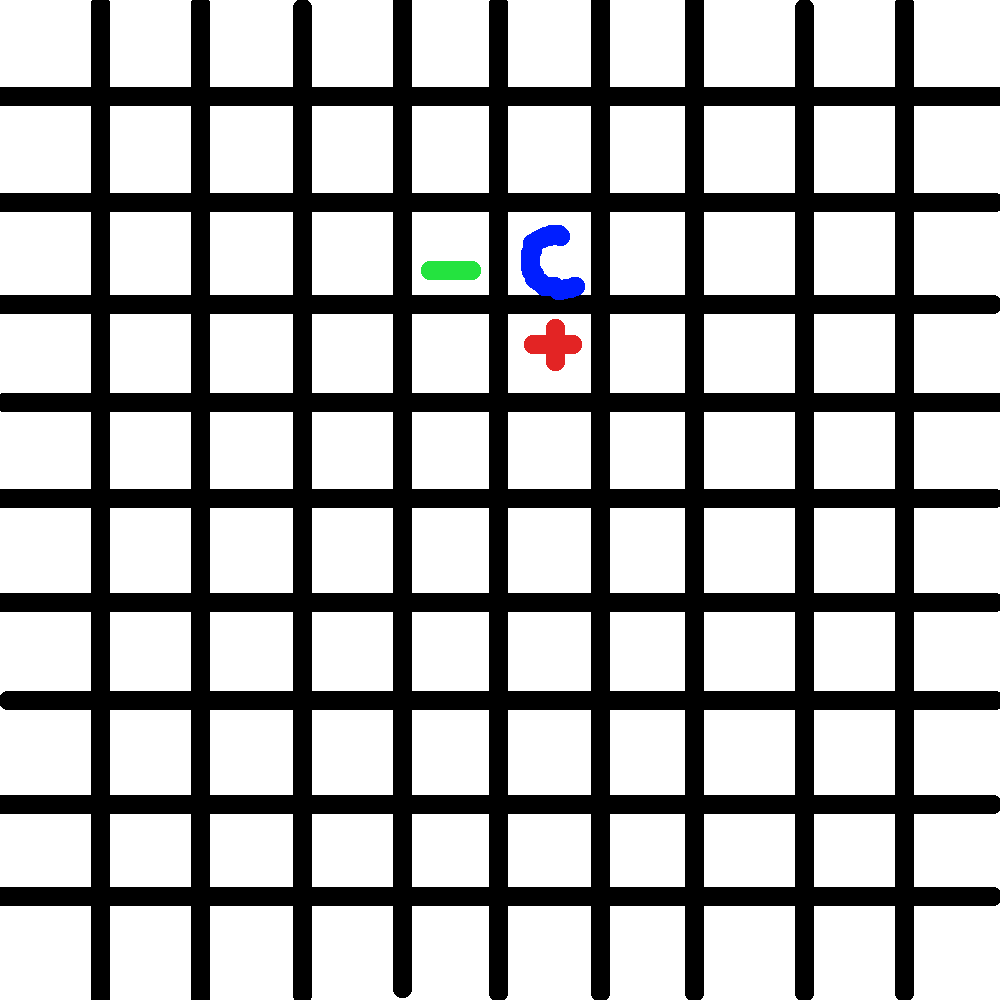
\includegraphics[scale=0.18]{grilla-casilla.png}\hfill }
\end{frame}

\begin{frame}{Optimización de Knuth (dibujos)}
    \begin{itemize}
		\item A lo largo de casi toda la matriz, los términos $K$ se cancelan.
        \item Las $N^2$ casillas pagan el término $1$: Total $O(N^2)$
        \item Las $O(N)$ casillas de borde pagan $O(|K|)$ Total $O(N|K|)$
    \end{itemize}
    {\hfill 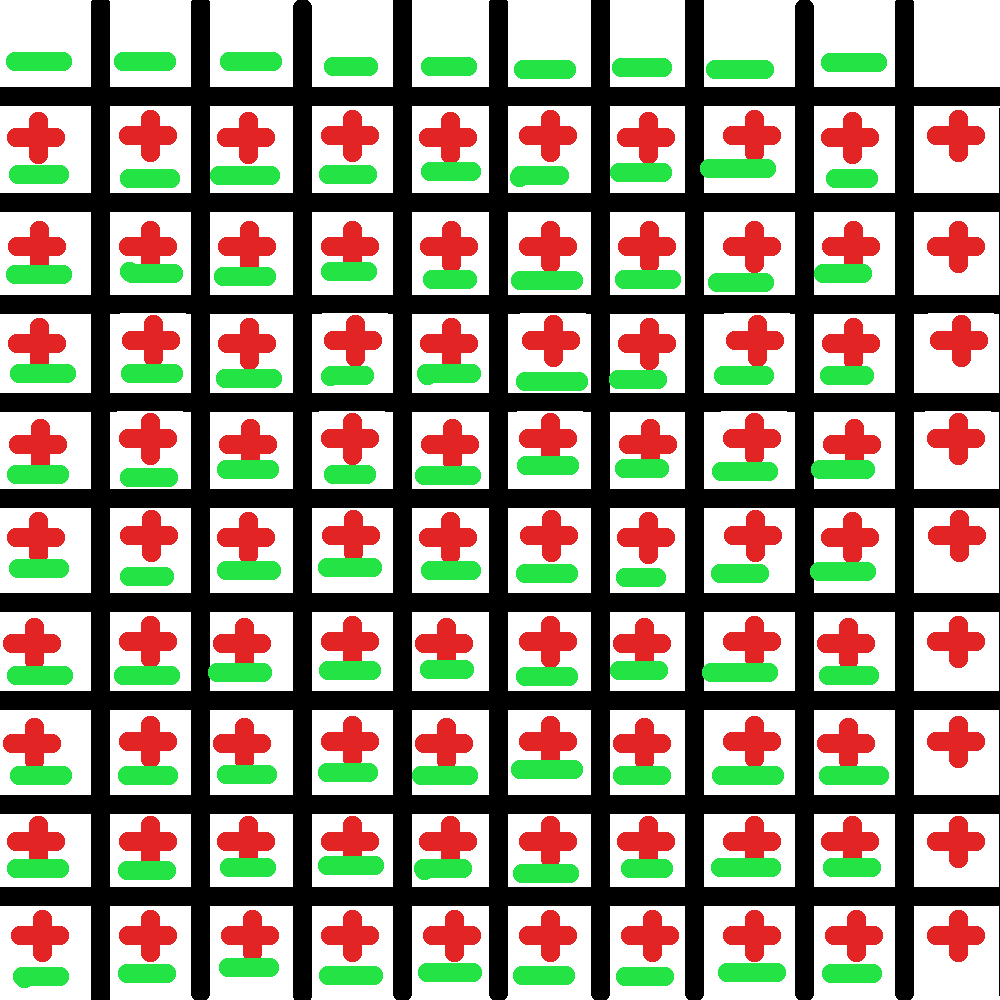
\includegraphics[scale=0.16]{grilla-cancelacion.png}\hfill }
\end{frame}

\begin{frame}{Comentarios}
    \begin{itemize}
        \item El dibujo muestra una matriz ``completa'' de $N \times N$
        \item La demostración aplica si ``borde'' $O(N)$ y tamaño $O(N^2)$
        \item Ejemplo: la parte triangular superior (dp en rangos)
    \end{itemize}
\end{frame}



\begin{frame}{Ejercicio}
    \begin{itemize}
		\item Ejercicio: Verificar que la condición de Knuth aplica en la recursión que vimos antes 
		\item Intuitivamente tiene muchísimo sentido, ¡pero demostrarlo es mucho más difícil que programarlo!
    \end{itemize}
\end{frame}


\subsection{Optimización de Divide and Conquer}

\begin{frame}{Ejemplo motivador}
    \begin{itemize}
		\item Dados $n$ valores $x_i$ enteros positivos, el costo de un intervalo $[i,j)$ es $\sum_{i \leq a<b<j}{x_a x_b} $. O sea, sumar los productos de a pares.
		\item Particionar el arreglo $[0,n)$ en $k$ intervalos, minimizando la suma de los $k$ costos.
		\pause
		\invisible<1>{
			\item $dp(n,k) = \mbox{min}_{i=0}^{n-1}{\ dp(i,k-1) + val(i,n)}$
			\item Complejidad: $O(N^2 K)$
			\item ¿Se podrá mejorar?
		}
    \end{itemize}
\end{frame}

\begin{frame}{Contexto}
    \begin{itemize}
		\item ¡Sí! Con la optimización de Divide and Conquer
		\item Dado un algoritmo de dp con dos parámetros, es decir \\ $dp(n,k)$ con $0 \leq n \leq N$ y $0 \leq k \leq K$
		\item Si su recursión tiene la forma $dp(n,k) = \underset{i}{\mbox{min}}{\ g(n,k,i)}$ para cierta $g$ que solo usa los $dp(j,k')$ con $k' < k$ 
		\item Podemos definir $I(n,k)$ como el menor $i$ en donde se alcanza el mínimo de la expresión para $dp(n,k)$
        \item Para escribir las complejidades, notaremos $|I|$ a la cantidad de valores posibles para $i$ en la expresión. Típicamente $|I|$ es aproximadamente $N$
    \end{itemize}
\end{frame}

\begin{frame}{Condición de Divide and Conquer}
    \begin{itemize}
		\item $I(n,k) \leq I(n+1,k)$
		\item Equivalentemente: $I$ es \textbf{monótona en n}.  
		\item En criollo para DPs de particionar: si para $k$ fijo agrando el rango, el último punto de corte también (mejor dicho: no retrocede) 
		\item Llamamos a la anterior la \textit{Condición de Divide and Conquer}
		\item Igual que antes, suele ser mucho más difícil demostrar que se cumple, que convencerse o intuir que así será
    \end{itemize}
\end{frame}

\begin{frame}{Optimización de Divide and Conquer}
    \begin{itemize}
		\item Esta optimización no es tan simple de implementar como la de Knuth, pero la idea también es sencilla.
		\item Supongamos que para calcular todos los $dp(n,k)$ para $k$ fijo, calculamos primero el $dp(n',k)$:
			\begin{itemize}
				\item Para los $n > n'$, alcanza con probar el $i$ \textbf{desde} $I(n',k)$ \\
						Es decir, no más de $L_1 = |I| - I(n',k) + 1$ valores
				\item Para los $n < n'$, alcanza con probar el $i$ \textbf{hasta} $I(n',k)$ \\
				        Es decir, no más de $L_2 = I(n',k) + 1$ valores
			\end{itemize}
		\item Esto nos parte el rango $[0,N)$ que debíamos calcular en dos restantes: $[0,n')$ y $[n'+1,N)$.
		\item En la primera parte hay que probar hasta $L_1$ valores, y en la segunda hasta $L_2$ valores.
    \end{itemize}
\end{frame}

\begin{frame}{Si profundizamos...}
    \begin{itemize}
		\item Podemos seguir partiendo estos rangos en dos recursivamente
		\item En el paso $k$ tendremos $2^k$ rangos, cada uno con hasta $L_i$ opciones factibles para el $i$.
		\item Observación: En cada paso, los $L_i$ suman $O(N + |I|)$
		\item Por lo tanto, procesar cada paso es $O(N + |I|)$
		\item Partiendo siempre a la mitad, serán $O(\lg N)$ pasos y la complejidad es $O((N + |I|) \lg N)$
		\item El algoritmo final cuesta $O(K(N+|I|)\lg N)$ evaluaciones de $g$
    \end{itemize}
\end{frame}



\begin{frame}{Ejercicio}
    \begin{itemize}
		\item Ejercicio: Verificar que la condición de Divide and Conquer aplica en la recursión que vimos antes 
		\item Pasa lo mismo que antes: Es más fácil intuirlo que probarlo
    \end{itemize}
\end{frame}

\begin{frame}{Resumen}
    Optimización de Knuth:
    \begin{itemize}
		\item Prototípico para DPs en rangos
		\item Punto óptimo debe ser monótono en ambas variables
        \item Requiere cuadrados o ``similares'': $O(N)$ borde, $O(N^2)$ estados
        \item Le saca un $|I|$ (ejemplo: $N^3 \rightarrow N^2$)
    \end{itemize}
    Optimización de Divide and Conquer:
    \begin{itemize}
		\item Prototípico para DPs ``de particionar''
		\item Punto óptimo debe ser monótono en una variable
        \item Cualquier forma (por ejemplo sirve aún si $K << N$)
        \item Cambia un $N|I|$ por $(N+|I|) \lg N$ (ejemplo: $KN^2 \rightarrow KN\lg N$)
    \end{itemize}
\end{frame}



\end{document}
